\section{Implementation}
\label{sec:implementation}

\subsection{Framework: Microsoft AutoGen}
AutoGen is a multi-agent framework developed by Microsoft. It offers natively a more flexible agent topology, enhanced LLM inference, and dynamic agent collaboration. These features enable us to build a more robust and flexible multi-agent system \cite{microsoft_autogen}.

These are the key components of AutoGen that we used in our project:
\begin{itemize}
    \item \textbf{ConversableAgent:} In AutoGen's framework, the ConversableAgent class serves as a customizable foundation for agents capable of engaging in conversations with other agents, humans, and tools to accomplish tasks collaboratively.
    \item \textbf{GroupChat:} A GroupChat is a collection of agents that can communicate with each other.
    \item \textbf{GroupChatManager:} In AutoGen's multi-agent group chat, the GroupChatManager plays a major role in facilitating agent communication. When an agent generates a response, the GroupChatManager broadcasts it to all participating agents in GroupChat. This broadcasting mechanism ensures that all agents remain informed of the ongoing conversation, allowing them to contribute effectively to collaborative tasks. The GroupChatManager also manages the flow of the conversation by selecting the next speaker, by orchestrating a coherent and organized dialogue among the agents.
    \item \textbf{SocietyOfMindAgent:} The Society of Mind Agent in Microsoft's AutoGen framework is inspired by Marvin Minsky's “Society of Mind” theory, which posits that intelligence emerges from the interactions of simple, mindless agents working together. In AutoGen, the Society of Mind Agent can orchestrate and wrap GroupChat and GroupChatManager objects that host agents and debates. Externally, it functions as a singular cohesive agent and the conversation within GroupChat under the SocietyOfMindAgent can be considered an "Inner Dialogue". This internal discourse allows for the weighing of options and the integration of multiple viewpoints, ultimately guiding behavior and thought processes.
\end{itemize}

\subsection{Code}
The code introduced a dynamic hierarchy system where a hierarchy string (e.g., “ABB”) defines the structure of a group of agents. Each letter in the hierarchy string represents the nodes that consists of agents such as the Prompt Generator, Counter, Working Agent, Checker, and Subordinate Nodes. The hierarchy system allows a clear definition of the agent hierarchy, a flexible representation of the topology, and an optimized information flow. 

\subsubsection{Agents}
\textbf{Prompt Generator:} The Prompt Generator is responsible for structuring and reformatting the problem before any agent attempts to solve it. It does not solve the problem itself but ensures that agents receive a clear and well-defined prompt.

\textbf{Counter:} The Counter Agent is responsible for tracking the number of debate rounds and ensuring the conversation does not continue indefinitely. It does not contribute to the discussion but simply counts rounds and signals progress.

\textbf{Working Agent:} The Working Agents are responsible for solving the problem based on the structured prompt. They generate initial solutions, review responses from other agents, and refine their answers through debate.

\textbf{Checker:} The Checker Agent is responsible for evaluating whether the Subordinate Agents' answers are converged. It does not solve the problem—instead, it decides whether the answers agree or if further rounds are needed. It can terminate or continue the debate based on the convergence of responses.

\textbf{Subordinate Nodes:} The Subordinate Nodes are nested within the SocietyOfMindAgent(s). These consist of the Prompt Generator, Counter, Working Agents, Checker, and Subordinate Nodes if these nodes host further subnodes. 

\subsubsection{Hierarchy String Conversion Rules}
The hierarchy string needs to be processed by a function to convert it into a multi-agent topology. The function is \textit{parse\_subnodes\_generic(letters)} that takes a string of letters as input and returns a list of subnodes. The function follows these rules:

\textbf{Rule 1: Identifying Generations (Levels of Hierarchy)}

The hierarchy is built by identifying distinct levels (generations) of agents, based on letter occurrences. The earliest occurring letter (lexicographically lowest) (e.g., 'A') is designated as Generation 0. Subsequent letters define child nodes of the previous generation, forming hierarchical relationships. Each new letter appearing after a previous letter indicates a transition to a lower level (subordinate node). 

For instance, the string is "ABC": $$"ABC" \rightarrow Gen\_0:A \rightarrow Gen\_1:B \text{(Subordinate to A)} \rightarrow Gen\_2:C \text{(Subordinate to B)}$$

\textbf{Rule 2: Grouping Subordinate Nodes}

For each identified generation, consecutive occurrences of the same letter are grouped under a common parent node. These grouped nodes operate within the same hierarchical layer and are peers within the structure.

\textbf{Rule 3: Parent-Child Relationships}

A letter that appears after another letter of the same or a lower level is assigned as its child. A new letter that appears after the lowest-ranked letter (earliest in order) indicates the start of a new group.

\textbf{Rule 4: Tracking Generations Dynamically}

The function dynamically tracks each letter’s depth in the hierarchy, ensuring that sibling nodes are grouped correctly, child nodes are assigned to the appropriate parent, and the overall hierarchical structure is accurately maintained.

\textbf{Rule 5: Handling Nested Hierarchies (Recursive Parsing)}

If a letter appears at a deeper level than its immediate predecessor, it belongs to a subordinate node. The function recursively parses the hierarchy to establish nested societies of mind.

\textbf{Rule 6: Assigning Subnode Identifiers}

Subordinate nodes are labeled with unique identifiers based on their structure. If a node is part of a repeated pattern, a numerical suffix is assigned to distinguish between different instances. If the string is "ABCCBCC", the subnode identifiers would be "ABB1" representing the first instance of BB under A, and "BCC1", and "BCC2" indicating two separate groups of BCC under different parent nodes.

\textbf{Example:}

Given the hierarchy string "ABCCBCCCABCDDCBCCDEEDEEC" and "ABCDEEDCDDDBCCBCDDCCB", the function would parse the hierarchy like these network diagrams in Figure ~\ref{fig:ABCCBCCCABCDDCBCCDEEDEEC} and Figure ~\ref{fig:ABCDEEDCDDDBCCBCDDCCB}

\begin{figure}[h]
    \centering
    \begin{minipage}{0.49\linewidth}
        \centering
        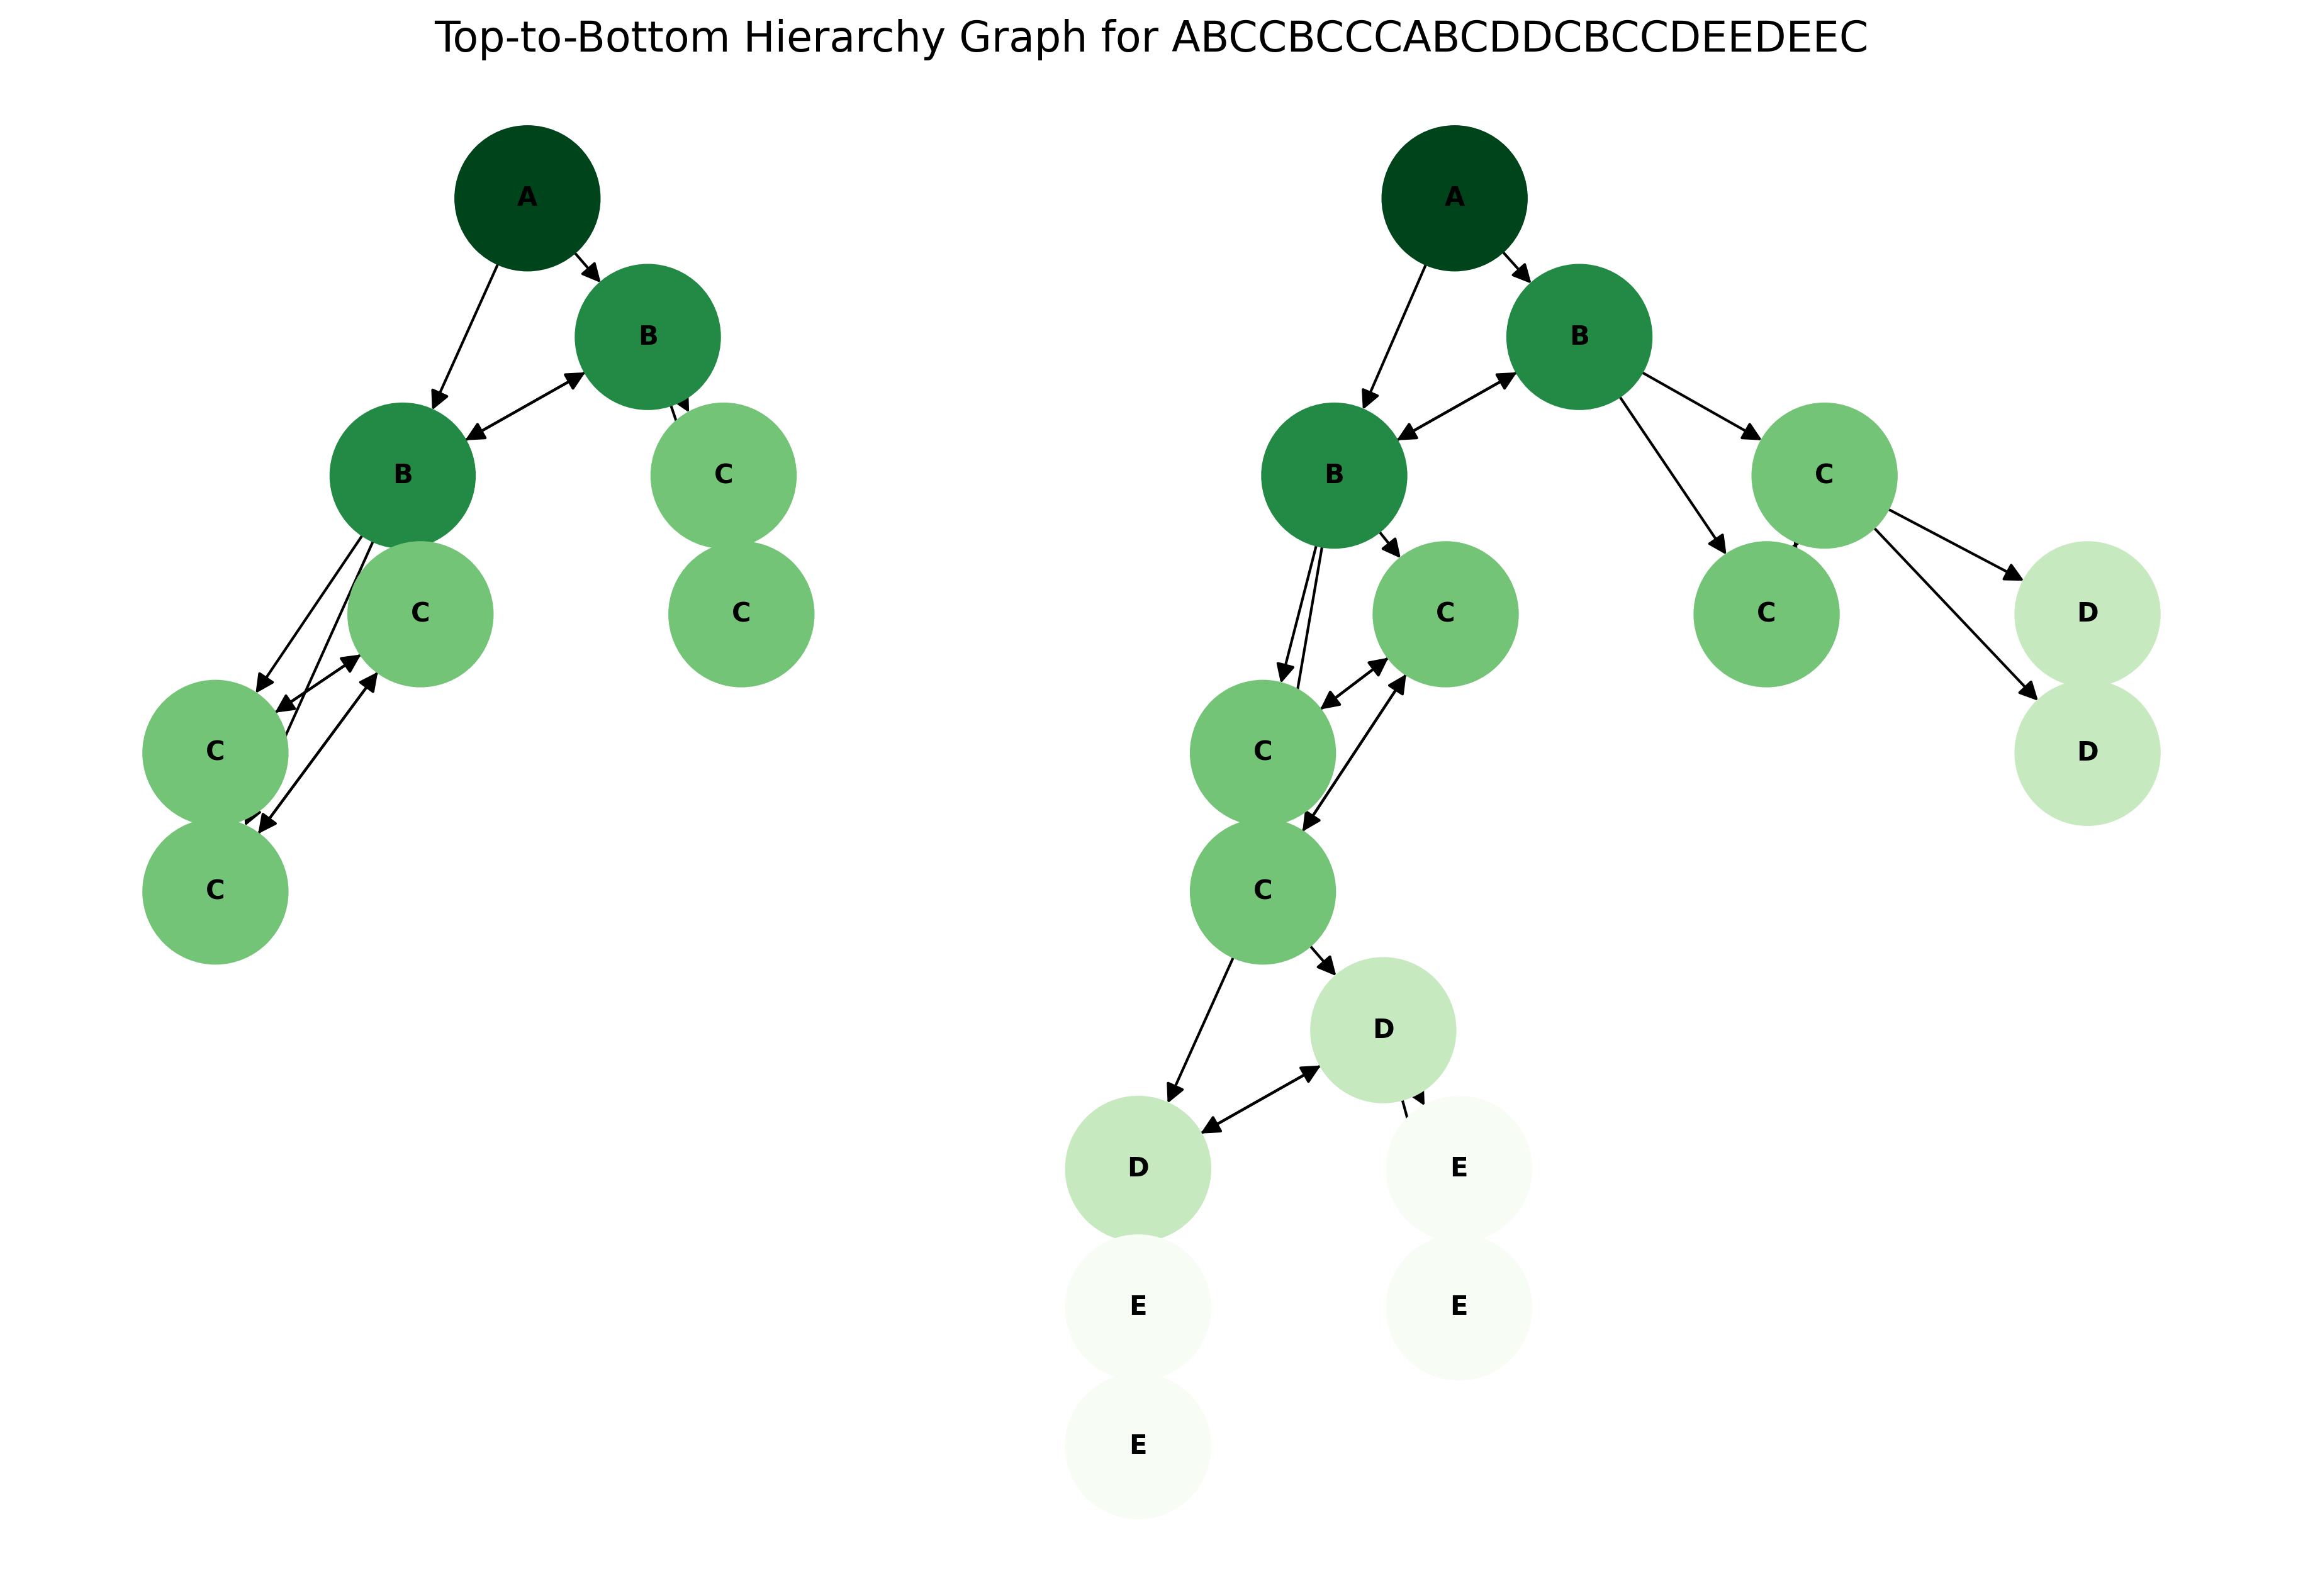
\includegraphics[width=\linewidth]{img/section_implement/ABCCBCCCABCDDCBCCDEEDEEC.png}
        \caption{Visualization of the hierarchy string "ABCCBCCCABCDDCBCCDEEDEEC"}
        \label{fig:ABCCBCCCABCDDCBCCDEEDEEC}
    \end{minipage}
    \hfill
    \begin{minipage}{0.49\linewidth}
        \centering
        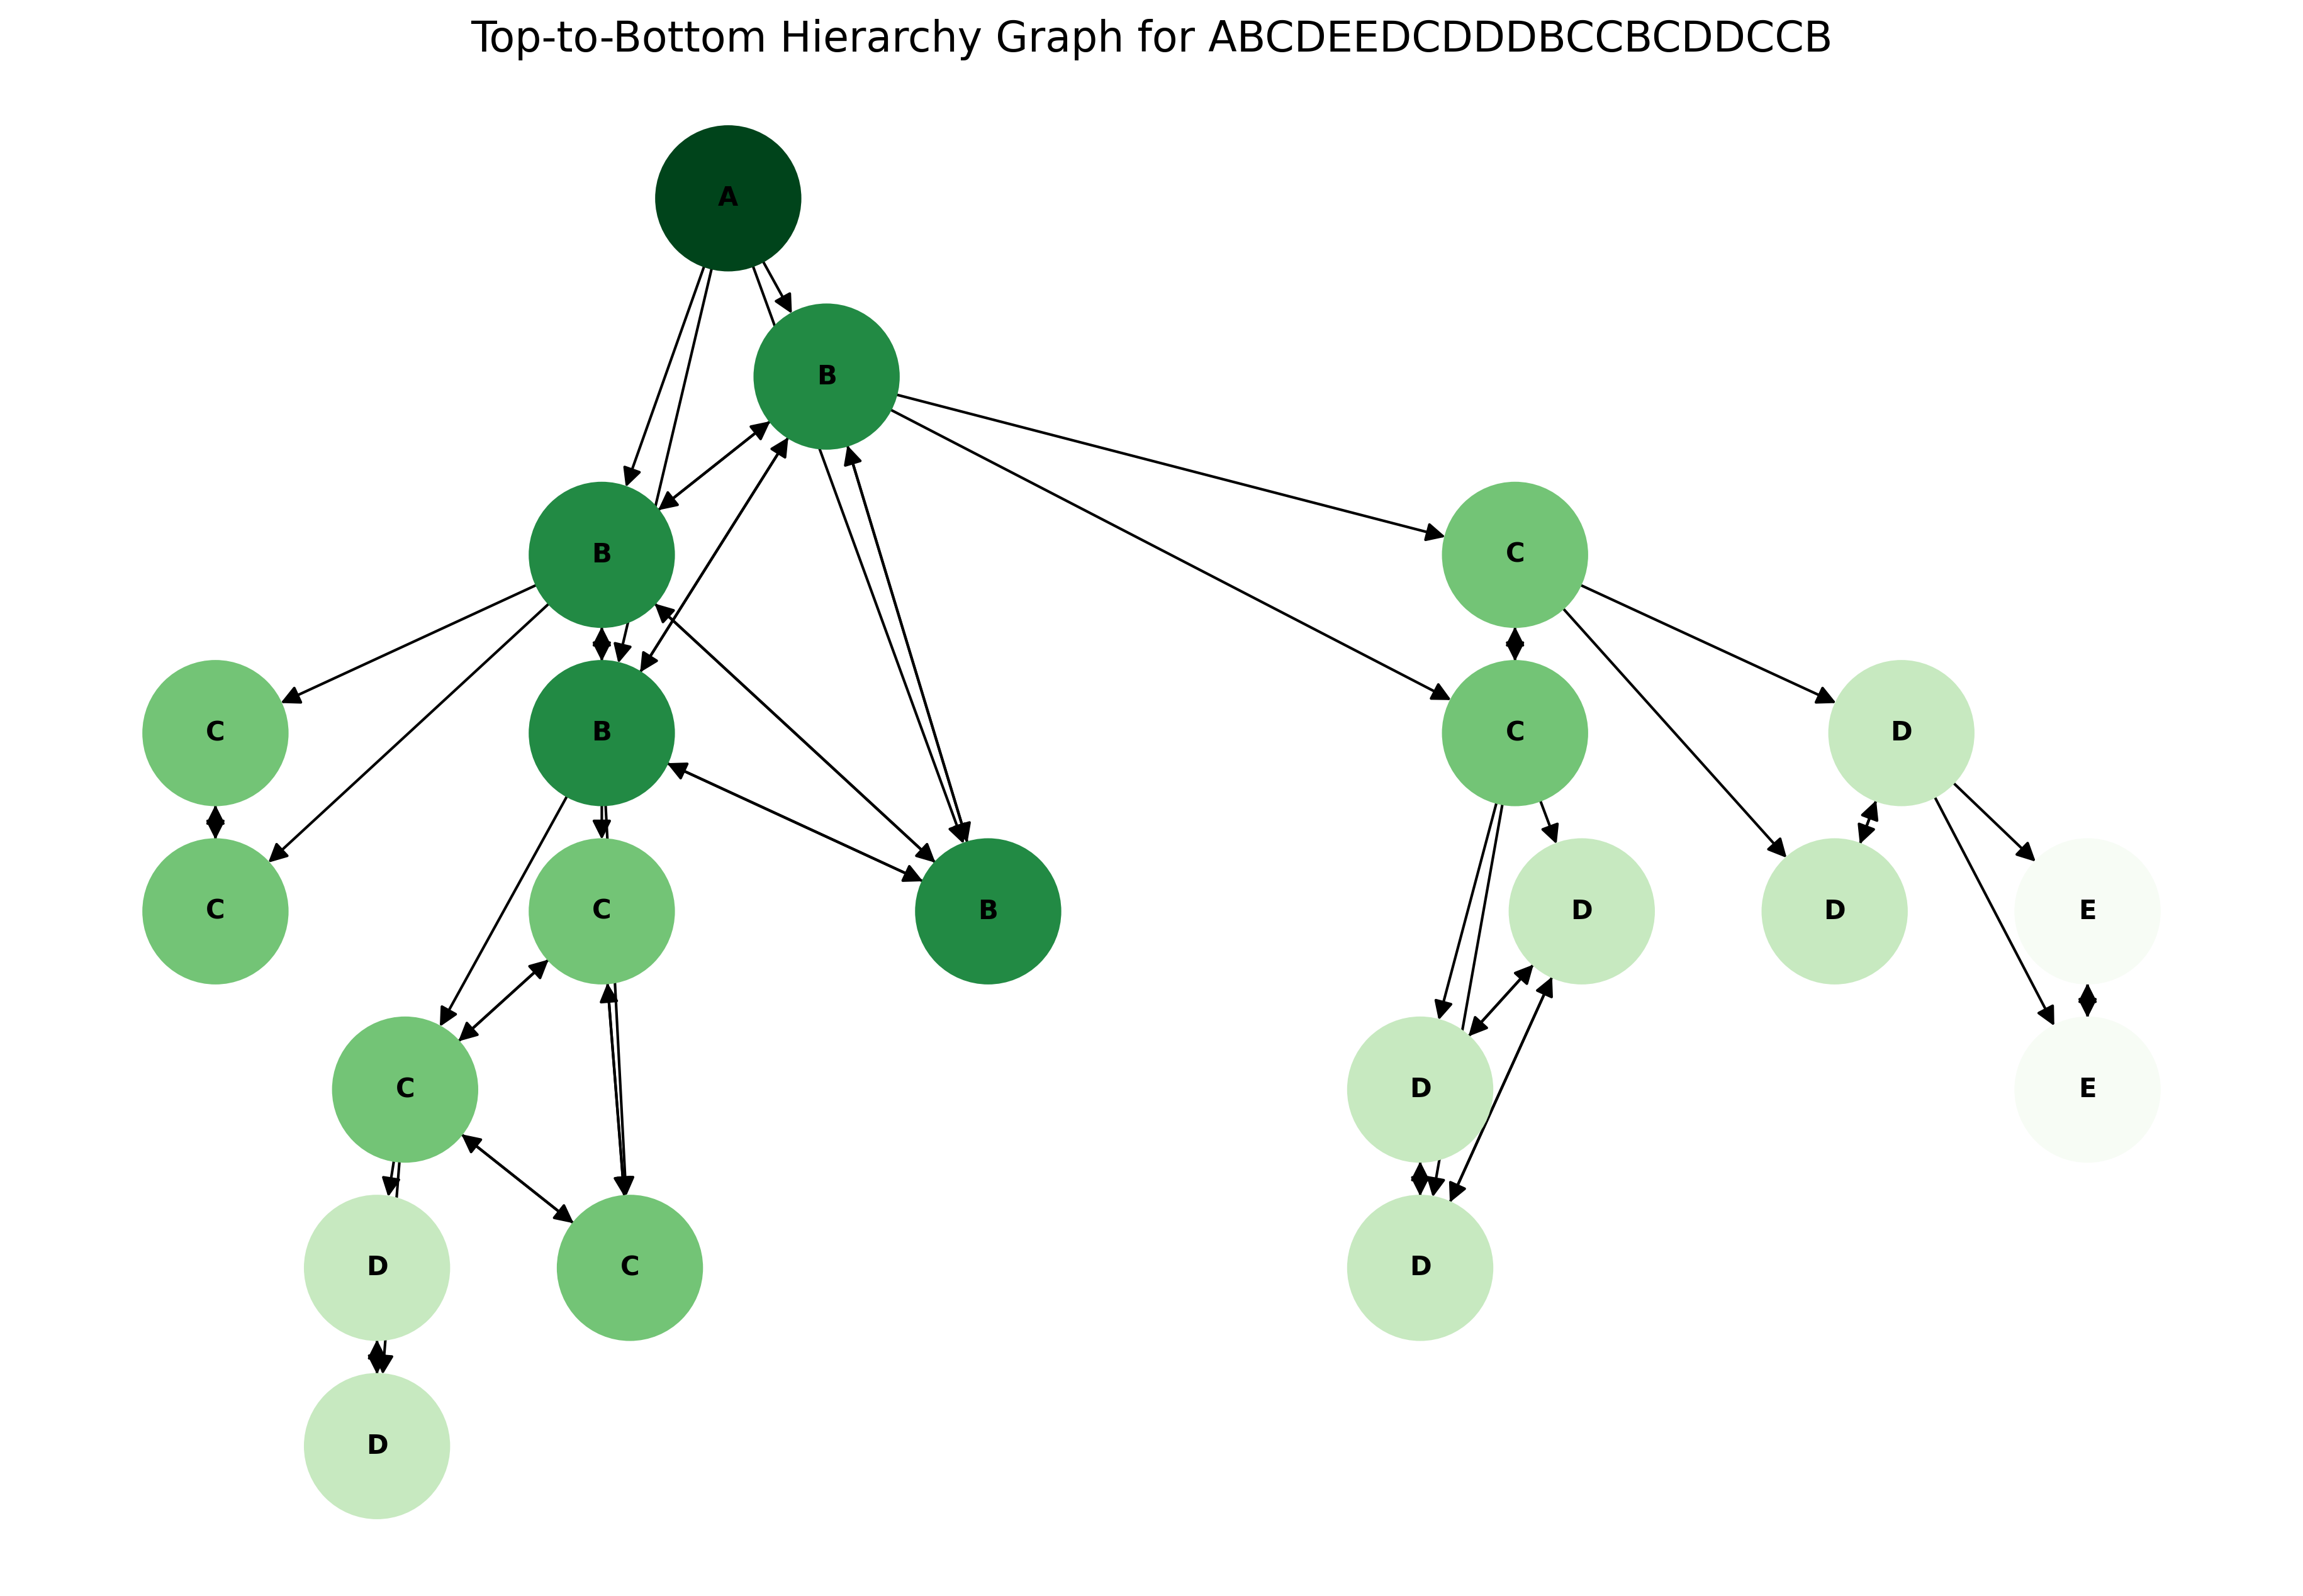
\includegraphics[width=\linewidth]{img/section_implement/ABCDEEDCDDDBCCBCDDCCB.png}
        \caption{Visualization of the hierarchy string "ABCDEEDCDDDBCCBCDDCCB"}
        \label{fig:ABCDEEDCDDDBCCBCDDCCB}
    \end{minipage}
\end{figure}

\subsubsection{Workflow}

The system operates by:
\begin{enumerate}
\item \textbf{Parsing the Hierarchy String:} The hierarchy string is processed to identify generations (Gen\_0, Gen\_1, ..., Gen\_i ..., Gen\_n), where each generation corresponds to a distinct group of agents.
\item \textbf{Forming Subnodes:} Each subnode is treated as an independent GroupChat, hosting its own set of agents (Prompt Generator, Counter, Working Agents, and Checker). These agents engage in structured discussions within their designated subnode. The nodes/subnodes are created dynamically based on the hierarchy string.
\item \textbf{Nested Debate and Refinement:} The debate starts at the lowest level (Gen\_0), where Working Agents produce initial solutions. As discussions progress, higher-generation (Gen\_i) subordinate subnodes generate the responses, leading to a hierarchical refinement of answers.
\item \textbf{Top-Down Control \& Bottom-Up Aggregation:} The Supreme Hierarchy SocietyOfMindAgent oversees the entire hierarchy, ensuring that responses from lower generations are aggregated and passed upwards, while high-level decisions cascade down to guide subnode debates.
\end{enumerate}

This hierarchical grouping approach optimizes communication, prevents redundant discussions across unrelated agents, and ensures that information flows efficiently between different levels of the system. The combination of structured debates, iterative refinement, and dynamic agent organization enables the framework to produce well-reasoned, high-quality, accurate responses.